%!TeX root=../tese.tex
%("dica" para o editor de texto: este arquivo é parte de um documento maior)
% para saber mais: https://tex.stackexchange.com/q/78101/183146

%% ------------------------------------------------------------------------- %%
\chapter{Interpretação geométrica de buscas em ABBs}
\label{cap:geometria}

Neste capítulo entenderemos o que são conjuntos de pontos arboreamente independente e como interpretar de maneira geométrica algoritmos de busca em ABBs..

\section{Conjuntos arboreamente satisfeitos}

Um par de pontos $(a,b)$ de um conjunto de pontos $P$ é \textit{arboreamente satisfeito} se $a$ e $b$ são ortogonalmente colineares ou se há pelo menos um ponto do conjunto \( P \setminus \{a,b\} \) que está dentro da área delimitada pelo retângulo de vértices $a$ e $b$, isto inclui o perímetro deste retângulo. Um conjunto $P$ de pontos é \textit{arboreamente satisfeito} se todos os pares de pontos do conjunto são arboreamente satisfeitos. Veja a Figura~\ref{fig:geometria-inicial}.

\begin{figure}[h!]
    \centering
    \begin{minipage}[b]{0.45\textwidth}
        \centering
        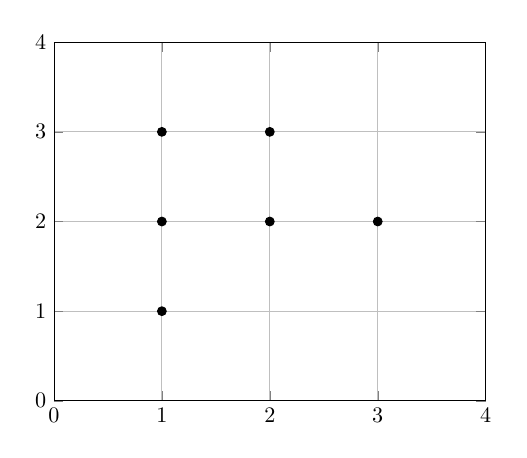
\begin{tikzpicture}[scale=0.8]
        \begin{axis}[
            grid=major,
            xmin=0, xmax=4,
            ymin=0, ymax=4,
            xtick={0,1,2,3,4},
            ytick={0,1,2,3,4}
        ]
        \addplot[only marks, mark=*] coordinates {
            (1,1)
            (1,2)
            (1,3)
            (2,2)
            (2,3)
            (3,2)
        };
        \end{axis}
        \end{tikzpicture}
    \end{minipage}\hfill
    \begin{minipage}[b]{0.45\textwidth}
        \centering
        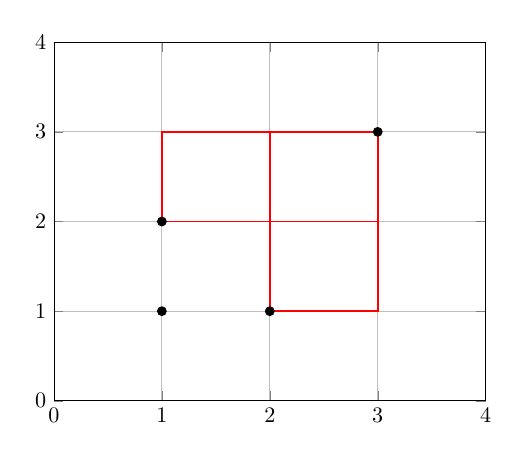
\begin{tikzpicture}[scale=0.8]
        \begin{axis}[
            grid=major,
            xmin=0, xmax=4,
            ymin=0, ymax=4,
            xtick={0,1,2,3,4},
            ytick={0,1,2,3,4}
        ]
        \addplot[only marks, mark=*] coordinates {
            (1,1)
            (1,2)
            (2,1)
            (3,3)
        };
        \addplot[
            color=red,
            line width=0.7pt
        ]
        coordinates {
            (2,1)
            (3,1)
            (3,3)
            (2,3)
            (2,1)
        };
        \addplot[
            color=red,
            line width=0.7pt
        ]
        coordinates {
            (1,2)
            (3,2)
            (3,3)
            (1,3)
            (1,2)
        };
        \end{axis}
        \end{tikzpicture}
    \end{minipage}
    \caption{À esquerda, um conjunto de pontos $P$ aboreamente satisfeito. À direita, um conjunto de pontos $P$ com dois pares de pontos aboreamente insatisfeitos com seus retângulos esboçados.}
\label{fig:geometria-inicial}
\end{figure}

\begin{lemma}
\label{lem:pontos_em_arestas_incidentes}
Em um conjunto arboreamento satisfeito, para todo par de pontos $(a,b)$ não ortogonalmente colineares, há sempre pelo menos um ponto de \( P \setminus \{a,b\} \) que está em alguma aresta que incide em $a$, e há sempre também pelo menos um ponto de \( P \setminus \{a,b\} \) que está em alguma aresta que incide em $b$.
\end{lemma}


\begin{figure}
    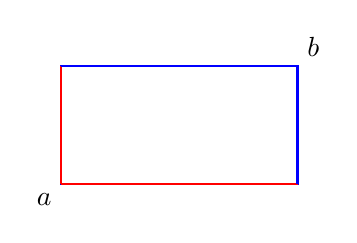
\begin{tikzpicture}[scale=1.5]
        \draw[blue, thick] (0,0) rectangle (2,1);
        
        \node at (0,0) [below left] {$a$};
        \node at (2,1) [above right] {$b$};
        
        \draw[red, thick] (0,0) -- (0,1);
        \draw[red, thick] (0,0) -- (2,0);
        \draw[blue, thick] (2,1) -- (0,1);
        \draw[blue, thick] (2,1) -- (2,0);
    \end{tikzpicture}
    \caption{Retângulo com vértices $a$ e $b$. Em vermelho estão destacadas as arestas do retângulo que incidem em $a$ e em azul estão destacadas as arestas que incidem em $b$.}
\end{figure}

\begin{proof} Sejam $a$ e $b$ dois pontos de um conjunto arboreamente satisfeito. Como $(a,b)$ é um par de pontos arboreamente satisfeitos, então a área delimitada pelo retângulo de vértices $a$ e $b$ possui pelo menos 1 ponto diferente de $\{a,b\}$. Denotemos por $c$ tal ponto. Se $c$ não estiver em uma aresta que incide em $a$, então é possível recursivamente procurar tal ponto no retângulo delimitado pelo par de pontos arboreamente satisfeitos $(a,c)$. Analogamente, se $c$ não estiver em uma aresta que incide em $b$, então é possível recursivamente procurar tal ponto no retângulo delimitado pelo par de pontos arboreamente satisfeitos $(c,b)$.
\end{proof}

%Seja $\tau_i$ a subárvore // falar de subarvores?

\section{Visão geométrica de buscas}

No modelo de computação adotado, para realizar um acesso em uma ABB, o algoritmo de busca inicia o nó corrente na raiz da ABB. Em seguida, este algoritmo percorre a árvore descendo para o filho apropriado por meio de comparações até alcançar a chave procurada.

Dada uma sequência $X = (x_{1},\ldots,x_{m})$ de $m$ acessos às chaves $x_{1}, x_{2},\ldots,x_{m}$, é possível ilustrar essa sequência $X$ de maneira gráfica em um plano cartesiano da seguinte forma: o eixo X representará as chaves armazenadas dentro da ABB e o eixo Y representará o tempo, ou seja, as buscas feitas nessa ABB. Assim, um ponto de coordenada ($x$,$y$) representa a busca da chave $x$ na ABB no instante de tempo $y$. Veja o exemplo da Figura~\ref{fig:busca_padrao}.

\begin{figure}
    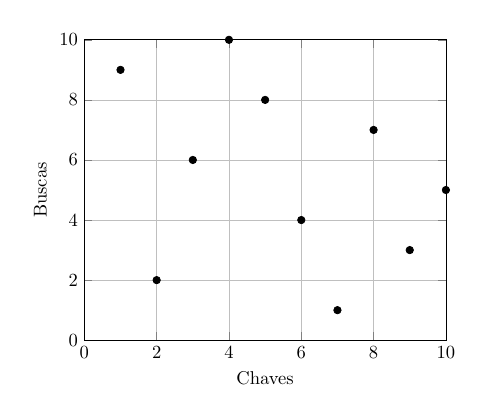
\begin{tikzpicture}[scale=0.67]
        \begin{axis}[
            xlabel={Chaves},
            ylabel={Buscas},
            grid=major,
            xmin=0, xmax=10,
            ymin=0, ymax=10,
            xtick={0,2,4,6,8,10},
            ytick={0,2,4,6,8,10}
        ]
        \addplot[only marks, mark=*] coordinates {
            (1,9)
            (2,2)
            (3,6)
            (4,10)
            (5,8)
            (6,4)
            (7,1)
            (8,7)
            (9,3)
            (10,5)
        };
        \end{axis}
    \end{tikzpicture}
    \caption{Gráfico representando a busca (7, 2, 9, 6, 10, 3, 8, 5, 1, 4).}
\label{fig:busca_padrao}
\end{figure}

A visão geométrica da execução de um algoritmo de busca em ABB para uma sequência $X = (x_{1},\ldots,x_{m})$ de buscas, de maneira similar, é o conjunto de pontos na forma ($x$,$y$) tal que $x$ foi uma chave acessada durante o instante de tempo $y$. É possível mapear esse conjunto de pontos para um plano cartesiano. Logo, todos os pontos com altura $y$ representam as chaves acessadas durante o instante de tempo $y$, ou seja, os nós acessados durante a busca por $x_y$. 
%não sei se eu gostei de $x_y$, porque $x$ é tanto coordenada quanto ponto na sequencia de busca

\begin{lemma} A visão geométrica de qualquer execução de um algoritmo de busca em ABB no modelo de computação adotado é um conjunto de pontos arboreamente satisfeitos.
\end{lemma}

\begin{proof}
Assuma que a visão geométrica de um algoritmo de busca em ABB não é arboreamento satisfeita. Dessa maneira, há pelo menos um par de pontos $(a,b)$ nesse conjunto que não é arboreamente satisfeito. Seja $a$ a chave buscada no instante de tempo $i$ e seja $b$ a chave buscada no instante de tempo $j$. Assumiremos também sem perda de generalidade que $i < j$ e $a < b$.

Seja $c$ o ancestral comum mais profundo de $a$ e $b$ imediatamente antes da busca $i$. E seja $d$ o acestral comum mais profundo de $a$ e $b$ imediatamente antes da busca $j$.

Denotaremos números para áreas específicas para simplificar a explicação da prova. 
Área 1 = \{$(x,y)$ | $x = a$ e $i < y \leq j$\}, representando todos os acessos a chave $a$ entre os instantes de tempo $i$ e $j$. \\
Área 2 = \{$(x,y)$ | $a \leq x < b$ e $y = j$\}, representando todos os acessos a chaves entre $a$ e $b$ no instante de tempo $j$. \\
Área 3 = \{$(x,y)$ | $x = b$ e $i \leq y < j$\}, representando todos os acessos a chave $b$ entre os instantes de tempo $i$ e $j$. \\
Área 4 = \{$(x,y)$ | $a < x \leq b$ e $y = i$\}, representando todos os acessos a chaves entre $a$ e $b$ no instante de tempo $i$. \\

Como $(a,b)$ não é um par de pontos arboreamente satisfeitos, nota-se que não há nenhum ponto tanto nas bordas quanto no interior do retângulo de vértices $a$ e $b$. Logo, $1 \cup 2 \cup 3 \cup 4 = \emptyset$.

Vale ressaltar que se $e$ é o ancestral comum mais profundo de $a$ e $b$, então sabemos que $a \leq e \leq b$ e mais importante, $e$ está mais acima na ABB em comparação com $a$ e $b$ (possivelmente na mesma profundidade caso seja igual a $a$ ou $b$). Assim, $e$ está no caminho da raiz da ABB até qualquer chave no intervalo $[a,b]$. Em outras palavras, para acessar qualquer chave no intervalo $[a,b]$, é necessário acessar o ancestral comum mais profundo entre $a$ e $b$.

\begin{figure}[H]
    \centering
    \vfill % Adiciona espaço acima da figura para centralização vertical
    \begin{minipage}[t]{0.6\textwidth}
        Se $2 = \emptyset$, então obrigatoriamente $d = b$. Se $c = b$, então $3 \neq \emptyset$. Se $c \neq b$, então em pelo menos algum outro instante de tempo $h$, $h < j$, $b$ teve que ser acessado para ser rotacionado até virar o ancestral comum mais profundo entre $a$ e $b$, logo $3 \neq \emptyset$.   

        Se $4 = \emptyset$, então $c = a$. Porém, no instante $j$, $b$ é acessado. Caso $c = d = a$, $a$ precisa ser acessado no instante de tempo $j$, logo $1 \neq \emptyset$. Caso $c \neq d$, então em algum instante de tempo $h$, $i \leq h < j$, o ancestral comum mais profundo entre $a$ e $b$ mudou, logo algum nó com chave no intervalo $(a,b]$ precisa ter sido rotacionado para cima, porém sabemos que para acessar qualquer chave no intervalo $[a,b]$ no instante de tempo $h$, é necesssário acessar o ancestral comum mais profundo que neste caso é $a$. Logo $1 \neq \emptyset$. 
    \end{minipage}\hfill
    \begin{minipage}[t]{0.4\textwidth}
        % Coluna da direita com a imagem e a legenda
        \centering
        \begin{figure}[H]
            \centering
            \begin{adjustbox}{valign=t, raise=-25pt} % Alinha o gráfico ao topo da caixa
            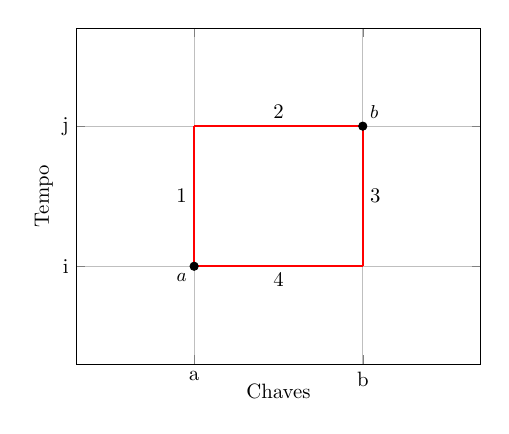
\begin{tikzpicture}[scale=0.75]
            \begin{axis}[
                xlabel={Chaves},
                ylabel={Tempo},
                grid=major,
                xmin=0.3, xmax=2.7,
                ymin=0.3, ymax=2.7,
                xtick={1,2},
                ytick={1,2},
                xlabel style={at={(axis description cs:0.5,-0.08)}, anchor=center}, % Ajusta a posição do rótulo do eixo x
                ylabel style={at={(axis description cs:-0.08,0.5)}, anchor=center},
                xticklabels={a,b}, % Define os rótulos do eixo x
                yticklabels={i,j} % Define os rótulos do eixo y
            ]

            \addplot[only marks, mark=*] coordinates {
                (1,1)
                (2,2)
            };

            \addplot[red, thick] coordinates {
                (1,2)
                (2,2)
            };

            \addplot[red, thick] coordinates {
                (2,2)
                (2,1)
            };

            \addplot[red, thick] coordinates {
                (1,1)
                (1,2)
            };

            \addplot[red, thick] coordinates {
                (1,1)
                (2,1)
            };

            % Adiciona rótulos aos pontos
            \node at (axis cs:1,1) [anchor=north east, fill=white, font=\small] {$a$};
            \node at (axis cs:2,2) [anchor=south west, fill=white, font=\small] {$b$};

            \node at (axis cs:1,1.5) [anchor=east, font=\normalsize] {1};
            \node at (axis cs:1.5,2) [anchor=south, font=\normalsize] {2};
            \node at (axis cs:2,1.5) [anchor=west, font=\normalsize] {3};
            \node at (axis cs:1.5,1) [anchor=north, font=\normalsize] {4};
            %\node at (axis cs:1.5,1.5) [anchor=center, font=\normalsize] {5};

            \end{axis}
            \end{tikzpicture}
            \end{adjustbox}
            \label{fig:tikz-captions}
        \end{figure}
    \end{minipage}
    \vfill % Adiciona espaço abaixo da figura para centralização vertical
    \label{fig:chaves-buscas}
\end{figure}

Por contrapositiva das conclusões acima, temos:
\begin{center}
Se $3 = \emptyset \Rightarrow 2 \neq \emptyset$. \\
Se $1 = \emptyset \Rightarrow 4 \neq \emptyset$.
\end{center}

Conclui-se então que $1 \cup 4  \neq \emptyset$ e $2 \cup 3  \neq \emptyset$, e assim chegamos numa contradição.

Vale ressaltar que é conveniente $1 \cup 4  \neq \emptyset$ e $2 \cup 3  \neq \emptyset$, uma vez que $1 \cup 4$ representa os pontos pertencentes as arestas do retângulo de vértices $a$ e $b$ incidentes ao vértice $a$ e  $2 \cup 3$ representa os pontos pertencentes as arestas incidentes ao vértice $b$. Assim, respeitando o Lema~\ref{lem:pontos_em_arestas_incidentes}.
\end{proof}

\begin{lemma}Qualquer conjunto de pontos arboreamente satisfeitos representa a execução de um algoritmo de busca em ABB no modelo de computação adotado.
\end{lemma}

\begin{proof}

Seja $N(x,i)$ o próximo acesso a chave $x$ depois do instante de tempo $i$.

É possível criar uma treap com nós que possuem a coordenada $x$ como chave. Além disso, usaremos o campo prioridade para representar o próximo instante de tempo que tal chave é acessada. As chaves são inicializadas como ($x$, $N(x,0)$) e no instante de tempo $t$ as chaves estão no formato ($x$, $N(x,t)$).

No instante de tempo $i$, os nós acessados, ou seja, todos os pontos do conjunto arboreamente satisfeito com coordenada $y=i$, formam uma subárvore que possui a raiz. Para reorganizar os nós de maneira a manter a propriedade heap da prioridade da treap para o instante de tempo $i+1$, é preciso reconfigurar os nós acessados de maneira a manter os nós mais superficiais como os nós que serão acessados mais cedo, ou seja, com menor $N(x,i)$. Na prática, após qualquer modificação de tempo é necessário reconfigurar a subárvore formada pelos pontos acessados como uma treap local.

Se conseguirmos manter a estrutura da treap após cada busca apenas acessando os elementos apropriados dados pelo conjunto arboreamente satisfeito, então evidentemente descrevemos um algoritmo offline que traduz um conjunto arboreamente satisfeito em um algoritmo de busca em ABB.

Vamos supor por contradição que não é possível manter a estrutura da treap entre o instante de tempo $i$ e $i+1$. Se não é possível manter tal estrutura, isso significa que há dois pontos, nomeados $a$ e $b$ ($a \neq b$), tal que $a$ está contido na subárvore dos vértices acessados no instante de tempo $i$ e $b$ não é acessado no instante de tempo $i$ e não consegue ser acessado no instante de tempo $i+1$ apenas com os pontos do conjunto arboreamente satisfeito. Assim, $N(a,i) > N(b,i)$. Assumiremos sem perda de generalidade que $a < b$ e $b$ é filho de $a$ na ABB durante o instante de tempo $i$. Veja a Figura~\ref{fig:representacao_grafica}.

De maneira informal, $a$ é um vértice que foi acessado no tempo $i$ e $b$ é o vértice filho de $a$ que por sua vez, não foi acessado no tempo $i$. O próximo acesso do vértice $b$ é mais cedo que o próximo acesso do vértice $a$. Para contradizer o lema, precisamos provar que um conjunto ser arboreamente satisfeito não é condição suficiente para garantir a manutenção da estrutura da treap de maneira adequada entre quaisquer instantes de tempo.

\begin{figure}
    \begin{tikzpicture}
        \coordinate (A) at (0, 0);
        \coordinate (B) at (3, 0);
        \coordinate (C) at (1.5, 2.6);
    
        \draw (A) -- (B) -- (C) -- cycle;
    
        \path (A) ++(0,1) coordinate (start);
        \path (start) ++(3,0.7) coordinate (end);
        \draw[dashed] (start) -- (end) node[midway,below] {};
    
        \path (start) ++(1.5,0.55) coordinate (x);
        \path (start) ++(1.7,0.2) coordinate (y);
    
        \filldraw (x) circle (2pt) node[anchor=south] {};
        \filldraw (y) circle (2pt) node[anchor=north] {};
    
        \draw[red, thick] (x) -- (y);
    
        \begin{scope}
            \clip (A) -- (B) -- (C) -- cycle; % Clipping para definir a área do triângulo
            \fill[pattern=vertical lines] (A) -- (C) -- (end) -- (start) -- cycle; % Preenchimento hachurado
        \end{scope}

        \filldraw (x) circle (2pt) node[anchor=south] {a};
        \filldraw (y) circle (2pt) node[anchor=north] {b};

        \draw[->, black] (1.8,1.8) -- (2.5,2) node[pos=1, right] {Chaves acessadas no instante de tempo $i$};
    \end{tikzpicture}
    \caption{Representação da situação descrita. Simplificação do formato de uma ABB por um triângulo, a área hachurada representa todos os nós acessados no instante de tempo $i$ e os nós $a$ e $b$ são nós pai-filho. O nó $b$ não foi acessado neste instante de tempo.}
\label{fig:representacao_grafica}
\end{figure}

Para simplificar a prova, denotaremos novamente números para áreas específicas: \\
Área 1 = \{$(x,y)$ | $x = a$ e $i < y \leq i+1$\}, representando todos os acessos a chave $a$ entre os instantes de tempo $i$ e $i+1$. \\
Área 2 = \{$(x,y)$ | $a < x \leq b$ e $y = i$\}, representando todos os acessos a chaves entre $a$ e $b$ no instante de tempo $i$.
Veja a Figura~\ref{fig:area_delimitada}.

\begin{figure}[H]
    \centering
    \begin{adjustbox}{valign=t, raise=-25pt} % Alinha o gráfico ao topo da caixa
    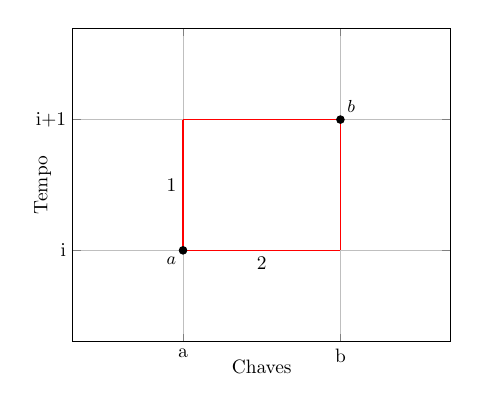
\begin{tikzpicture}[scale=0.7]
    \begin{axis}[
        xlabel={Chaves},
        ylabel={Tempo},
        grid=major,
        xmin=0.3, xmax=2.7,
        ymin=0.3, ymax=2.7,
        xtick={1,2},
        ytick={1,2},
        xlabel style={at={(axis description cs:0.5,-0.08)}, anchor=center}, % Ajusta a posição do rótulo do eixo x
        ylabel style={at={(axis description cs:-0.08,0.5)}, anchor=center},
        xticklabels={a,b}, % Define os rótulos do eixo x
        yticklabels={i,i+1} % Define os rótulos do eixo y
    ]

    \addplot[only marks, mark=*] coordinates {
        (1,1)
        (2,2)
    };

    \addplot[red, thick] coordinates {
        (1,2)
        (2,2)
    };

    \addplot[red, thick] coordinates {
        (2,2)
        (2,1)
    };

    \addplot[red, thick] coordinates {
        (1,1)
        (1,2)
    };

    \addplot[red, thick] coordinates {
        (1,1)
        (2,1)
    };

    % Adiciona rótulos aos pontos
    \node at (axis cs:1,1) [anchor=north east, fill=white, font=\small] {$a$};
    \node at (axis cs:2,2) [anchor=south west, fill=white, font=\small] {$b$};

    \node at (axis cs:1,1.5) [anchor=east, font=\normalsize] {1};
    \node at (axis cs:1.5,1) [anchor=north, font=\normalsize] {2};
    %\node at (axis cs:1.5,1.5) [anchor=center, font=\normalsize] {5};

    \end{axis}
    \end{tikzpicture}
    \end{adjustbox}
    \caption{Representação geométrica da área delimitada pelo retângulo de vértices $a$ e $b$.}
\label{fig:area_delimitada}
\end{figure}

De acordo com o Lema~\ref{lem:pontos_em_arestas_incidentes}, como $(a,b)$ representa um par de pontos arboreamente satisfeitos, então há pelo menos um outro ponto em alguma das arestas que incide em $a$. Como $N(a,i) > N(b,i)$, então sabemos que a área 1 não possui pontos no conjunto arboreamente satisfeito. Logo, para o Lema~\ref{lem:pontos_em_arestas_incidentes} ser verdadeiro, alguma chave entre $a$ e $b$ deve ter sido acessada no instante de tempo $i$, ou seja, $2 \neq \emptyset$. 

Como $b$ é filho direito de $a$, então para acessar qualquer chave no intervalo ($a,b$) no instante de tempo $i$, pela propriedade de ordenação de ABBs, é necessário acessar a chave $b$, pois as chaves neste intervalo são mais profundas que $a$ e $b$. Porém a suposição inicial era que $b$ não foi tocado no instante de tempo $i$, logo chegamos numa contradição.

Assim, nota-se que a reestruturação da treap da maneira proposta é sempre válida em conjuntos de pontos arboreamente satisfeitos e tal reestruturação é um algoritmo offline que converte um conjunto de pontos arboreamente satisfeitos em uma execução de um algoritmo de busca em ABB.
\end{proof}

